%%%%%%%%%%%%%%%%%%%%%%%%%%%%%%%%%%%%%%%%%%%%%%%%%%%%%%%%%%%%%%%%%%%%%%
% LaTeX Template: Curriculum Vitae
%
% Source: http://www.howtotex.com/
% Feel free to distribute this template, but please keep the
% referal to HowToTeX.com.
% Date: July 2011
% 
%%%%%%%%%%%%%%%%%%%%%%%%%%%%%%%%%%%%%%%%%%%%%%%%%%%%%%%%%%%%%%%%%%%%%%
\documentclass[paper=a4,fontsize=10.5pt]{scrartcl} % KOMA-article class
							
%\usepackage[english]{babel}
%\usepackage{CJKutf8}
%\usepackage[utf8x]{inputenc}
\usepackage[protrusion=true,expansion=true]{microtype}
%\usepackage{amsmath,amsfonts,amsthm}     % Math packages
\usepackage{graphicx}                    % Enable pdflatex
\usepackage[svgnames]{xcolor}            % Colors by their 'svgnames'
\usepackage{geometry}
	\textheight=900px                    % Saving trees ;-)
\usepackage{url}
\usepackage{wrapfig}
\usepackage{pxrubrica}
\usepackage[whole]{bxcjkjatype}

\usepackage{fancyhdr}
\setlength{\headheight}{0pt}
\setlength{\voffset}{-0.3in}
\setlength{\headsep}{5pt}
%\pagestyle{fancy}

\frenchspacing              % Better looking spacings after periods
%\pagestyle{empty}           % No pagenumbers/headers/footers
%\thispagestyle{plain}

%%% Custom sectioning (sectsty package)
%%% ------------------------------------------------------------
\usepackage{sectsty}

\sectionfont{%			            % Change font of \section command
	\usefont{OT1}{phv}{b}{n}%		% bch-b-n: CharterBT-Bold font
	\sectionrule{0pt}{0pt}{-5pt}{3pt}}

%%% Macros
%%% ------------------------------------------------------------
\newlength{\spacebox}
\settowidth{\spacebox}{8888888888}			% Box to align text
\newcommand{\sepspace}{\vspace*{0em}}		% Vertical space macro

\newcommand{\MyName}[1]{ % Name
		\LARGE \usefont{OT1}{phv}{b}{n} \hfill #1
		\par \normalsize \normalfont}
		
\newcommand{\MySlogan}[1]{ % Slogan (optional)
		\LARGE \usefont{OT1}{phv}{m}{n}\hfill \textit{#1}
		\par \normalsize \normalfont}

\newcommand{\NewPart}[1]{\section*{\uppercase{#1}}}

\newcommand{\PersonalEntry}[2]{
		\noindent\hangindent=2em\hangafter=0 % Indentation
		\parbox{\spacebox}{        % Box to align text
		\textit{#1}}		       % Entry name (birth, address, etc.)
		\hspace{1.5em} #2 \par}    % Entry value

\newcommand{\SkillsEntry}[2]{      % Same as \PersonalEntry
		\noindent\hangindent=2em\hangafter=0 % Indentation
		\parbox{\spacebox}{        % Box to align text
		\textit{#1}}			   % Entry name (birth, address, etc.)
		\hspace{1.5em} #2 \par}    % Entry value	
		
\newcommand{\EducationEntry}[4]{
		\noindent \textbf{#1} \hfill      % Study
		\colorbox{Black}{%
			\parbox{7em}{%
			\hfill\color{White}#2}} \par  % Duration
		\noindent \textit{#3} \par        % School
		\noindent\hangindent=2em\hangafter=0 \small #4 % Description
		\normalsize \par}

\newcommand{\WorkEntry}[4]{				  % Same as \EducationEntry
		\noindent \textbf{#1} \hfill      % Jobname
		\colorbox{Black}{\color{White}#2} \par  % Duration
		\noindent \textit{#3} \par              % Company
		\noindent\hangindent=2em\hangafter=0 \small #4 % Description
		\normalsize \par}

%%% Begin Document
%%% ------------------------------------------------------------
\begin{document}
% you can upload a photo and include it here...
\begin{wrapfigure}{l}{0.5\textwidth}
	\vspace*{-3.25em}
		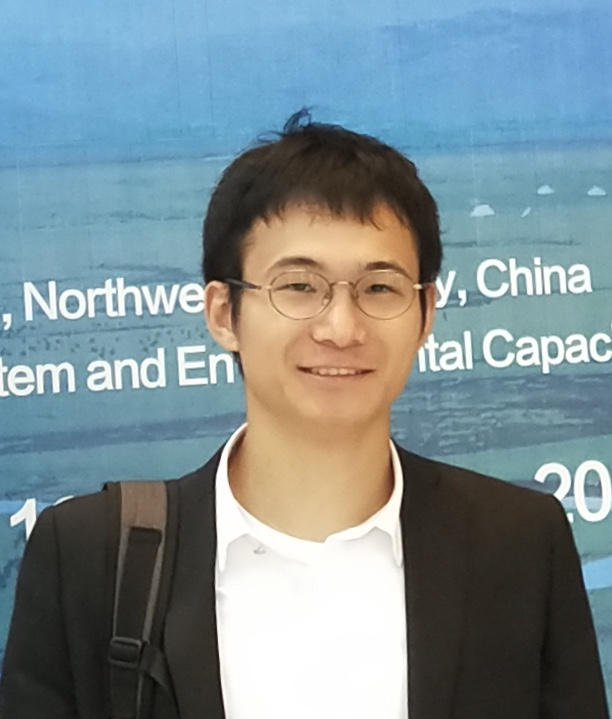
\includegraphics[width=0.15\textwidth]{./photo.jpg}
\end{wrapfigure}

%\MyName{\begin{CJK}{UTF8}{ipxm}\ruby{盧}{る} \ \ \  \ruby{涛}{たお}\end{CJK}}
%\MySlogan{\begin{CJK}{UTF8}{ipxm}履歴書\end{CJK}}
\MyName{\ruby{Lu}{る} \ \ \  \ruby{Tao}{たお}}
\MySlogan{履\ \ 歴\ \ 書}

%\sepspace

%%% Personal details
%%% ------------------------------------------------------------
\vspace{-0.5\baselineskip}
\NewPart{個人情報}{}

\PersonalEntry{誕生日}{1992年1月6日}
\PersonalEntry{住所}{東京都練馬区大泉学園町1-2-6 エメラルドII 202号室}
%\PersonalEntry{}{Midori Ku, Sagamihara City, Kanagawa}
\PersonalEntry{携帯}{(081) 070-2188-7509}
\PersonalEntry{メール}{\url{tao4free@gmail.com}}

%%% Education
%%% ------------------------------------------------------------
\vspace{-1.1\baselineskip}
\NewPart{学歴}{}

\EducationEntry{修士 都市環境学}{2015年-2017年}{中央大学 日本}{国際水環境理工学人材育成プログラムに参加。様々な水資源災害問題および解決に関するコースを経て、問題解決能力を伸ばすことができました。研究テーマはWRF を用いた短時間豪雨予測システムの構築に関する基礎研究でした。研究の際にLinux環境を用いてデータ処理および可視化の能力が鍛えられた。プログラミングおよびIT技術に関心を深めた。}
\sepspace
\vspace*{0.3em}

\EducationEntry{学士 港口水路及海岸工学}{2010年-2014年}{河海大学 中国}{Fortranを用いて有効波高の計算プログラムで初めてプログラミングに興味を持つようになりました。}

%%% Publications
%%% ------------------------------------------------------------
\vspace{-1.1\baselineskip}
\NewPart{論文}{}
Tao Lu, Tomohito Yamada, and Tadashi Yamada. "Fundamental Study of Real-time Short-term Rainfall Prediction System in Watershed: Case Study of Kinu Watershed in Japan." Procedia Engineering 154 (2016): 88-93.  

%%% Work experience
%%% ------------------------------------------------------------
\vspace{-1.1\baselineskip}
\NewPart{職\ 歴}{}

\EducationEntry{ソリューション事業部}{2017年-2019年}{株式会社地圏環境テクノロジー 正社員}{3次元水文地質モデルを構築し、水資源および水災害に関する受託解析を行っており、資源環境管理のソリューションを提供します。今は鉱山の坑廃水処理の業務に携わっております。仕事を通してチームワークおよびスケジュール管理の能力を身につけました。チームワークの際にコミュニケーションをきっちりとることは社内成果・サービスの提供、顧客の満足につながる重要な一環です。}
%\sepspace


%%% Skills
%%% ------------------------------------------------------------
\vspace{-1.1\baselineskip}
\NewPart{スキル}{}

\SkillsEntry{言語}{中 国 語 (母語)}
\SkillsEntry{}{英   語 (流暢)}
\SkillsEntry{}{日 本 語 (流暢, N1)}
\SkillsEntry{}{スペイン語 (初心者)}

\SkillsEntry{プログラム}{Python:国土交通省等のデータダウンロードツールの作成経験、}
\SkillsEntry{}{QGISのプラグイン開発経験(SuperLabeling:4039 ダウンロード)}
\SkillsEntry{}{\textsc{fortran:}データ処理}
\SkillsEntry{}{\textsc{html:}\url {https://tao4free.github.io/Hydrology/}}


%%% Experiences
%%% ------------------------------------------------------------
\vspace{-1.1\baselineskip}
\NewPart{ほかの経験}{}
1. アメリカのUCDavisで1ヶ月短期留学(その間、技術発表の訓練及び実践を行いた)\\
2. 2回国際学会経験 (International Conference on Hydroinformatics (HIC 2016); ISEWS2018)

%%% Experiences
%%% ------------------------------------------------------------
\vspace{-1.1\baselineskip}
\NewPart{志望職}{}
1. システムズエンジニア(SE)\\
2. ネットワークコンサルティングエンジニア(NCE) \\
3. カスタマーサポートエンジニア(CSE)

\end{document}
